\subsection{Mismatched Crowdsourcing}
\label{sec:MC}

%\begin{figure}
%  \centerline{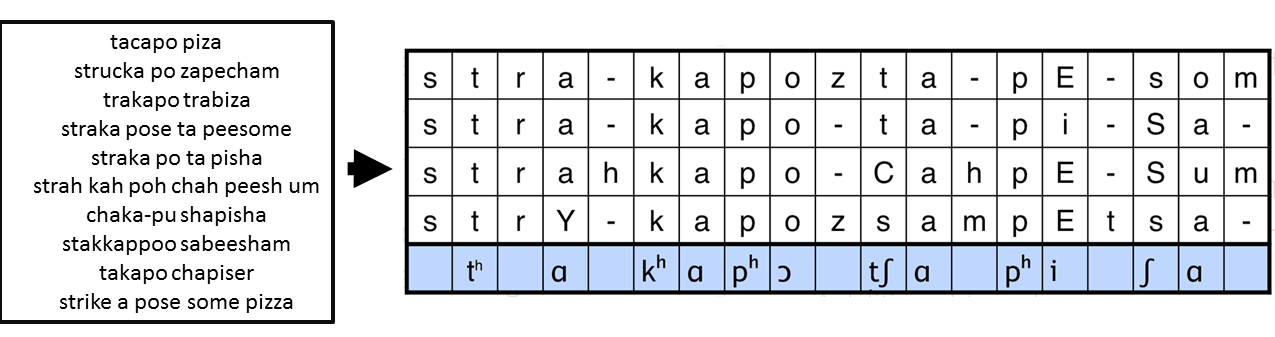
\includegraphics[width=5in]{../figs/fig_jyothi.png}}
%  \caption{In mismatched crowdsourcing, people who don't speak a
%    language (in this case Swahili) are asked to transcribe it using
%    nonsense syllables in the orthography of their own language (in
%    this case English).  There is a great deal of variability in their
%    responses (left), but information about the phonetic content of
%    the speech can be derived by merging the transcripts (top four
%    rows at right) and decoding using a model of non-native speech
%    perception (decoding result in the bottom row at right).}
%  \label{fig:mc}
%\end{figure}
%% comments: it's odd that all four of the illustrated transcripts begin
%% with the sequence [str], but the decoded result does not include the
%% [s] or the [r]. Perhaps it would be better to choose four transcripts
%% that vary more widely (and even indicate which orthographic strings
%% they correspond to) so that the derived result looks more plausible.
%% It is also odd that the formation of lambda involves choosing 5 best
%% MTs, but the figure shows 4 MTs.
%% Also, it is odd that pseudo-phonetic code is used in the transcripts
%% instead of IPA; IPA only occurs in the decoded result. Is there a
%% compelling reason for that?  Also, this figure is an excellent
%% candidate for vector graphic format rather than raster, since it's
%% all lines and text. I'm happy to help out with recreating figures in
%% vector format if that's desired.
%% Finally, I think this figure belongs after the following paragraph,
%% which could sensibly be merged into the opening paragraph of this
%% section. 

\begin{figure}[b!]\setlength{\textfloatsep}{3mm}
\begin{center}
  \tikzstyle{pre}=[<-,shorten <=3pt,>=stealth',thick, draw=black]
  \tikzstyle{post}=[->,shorten >=3pt,>=stealth',thick, draw=black]
  \begin{tikzpicture}[
      boxed/.style={rectangle,thick, draw=black, text=black, rounded corners=1mm, text centered, text width=5cm},
      state/.style={circle,thick, draw=black, text=black, text width=0.25cm},
      open/.style={text=black, text centered, text width=2.75cm},
    ]
    \node[boxed] (n0) at (0,0) {\begin{tiny}\begin{tabular}{c}$T$=Transcriptions\\\hline piza\\zapecham\\trabiza\\ta peesome\\ta pisha\\chah peesh um\\shapisha\\sabeesham\\chapiser\\some pizza\end{tabular}\end{tiny}};
    \node[boxed] (n1) at (6,0) {\begin{tiny}\begin{tabular}{c}$\rho(\lambda|T)=$Orthographic Confusion Network\\\hline\vspace{3cm}\end{tabular}\end{tiny}} edge[pre] (n0);
    \node[state] (g0) at (4,-0.25) {};
    \node[state] (g1) at (5.75,-0.25) {};
    \draw[post] (g0) -- (4.25,0.75) -- (5.25,0.75) -- (g1);
    \node at (4.75,1) {\tiny $<$t$>$$/0.4$};
    \draw[post] (g0) -- (4.25,-0.25) -- (5.25,-0.25) -- (g1);
    \node at (4.75,0) {\tiny $<$ch$>$$/0.4$};
    \draw[post] (g0) -- (4.25,-1.25) -- (5.25,-1.25) -- (g1);
    \node at (4.75,-1) {\tiny $<$s$>$$/0.2$};
    \node[state] (g2) at (7.5,-0.25) {};
    \draw[post] (g1) -- (g2);
    \node at (6.5,0) {\tiny $<$a$>$$/1.0$};
    \node[open] at (8.25,-0.25) {\ldots};
    \node[boxed] (n2) at (12,0) {\begin{tiny}\begin{tabular}{c}$\rho(\phi|T)=$Phone Confusion Network\\\hline\vspace*{3cm}\end{tabular}\end{tiny}} edge[pre] (n1);
    \node[state] (g10) at (10,-0.25) {};
    \node[state] (g11) at (11.75,-0.25) {};
    \draw[post] (g10) -- (10.25,0.75) -- (11.25,0.75) -- (g11);
    \node at (10.75,1) {\tiny \ipa{[t]}$/0.4$};
    \draw[post] (g10) -- (10.25,-0.25) -- (11.25,-0.25) -- (g11);
    \node at (10.75,0) {\tiny \ipa{[tS]}$/0.4$};
    \draw[post] (g10) -- (10.25,-1.25) -- (11.25,-1.25) -- (g11);
    \node at (10.75,-1) {\tiny \ipa{[s]}$/0.2$};
    \node[state] (g12) at (13.5,-0.25) {};
    \draw[post] (g11) -- (g12);
    \node at (12.5,0) {\tiny \ipa{[A]}$/1.0$};
    \node[open] at (14.25,-0.25) {\ldots};
  \end{tikzpicture}\\
\end{center}
\setlength{\abovecaptionskip}{0pt}
\caption{Probabilistic transcription from mismatched crowdsourcing:
  Transcripts $T$ are filtered to remove outliers, and merged to
  create a confusion network over orthographic symbols,
  $\rho(\lambda|T)$, from which the probabilistic transcription
  $\rho(\phi|T)$ is inferred. Example shown: Swahili speech,
  English-speaking transcribers.  Symbols in $<$$>$ are graphemes,
  symbols in $[]$ are phones, numbers are probabilities.}
\label{fig:mcmethods}
\end{figure}

The second set of PTs were computed by sending audio in the target
language to non-speakers of the target language, and asking them to
write what they hear.  It would be preferable to recruit transcribers
who speak a language with predictable orthography, but since
transcribers in those languages were not readily available, this
experiment instead recruited transcribers who speak American English.
Denote using $T$ the set of text
transcripts produced by these English-speaking crowd workers.
Mismatched transcripts must be converted into the form of a pmf over
target-language phone sequences, $\rho(\phi|T)$.  As an intermediate
step towards this goal, prior work~\cite{JHJ15b} developed techniques
to merge the transcripts in $T$ into a confusion network
$\rho(\lambda|T)$ over representative crowd-worker transcripts,
denoted $\lambda$ (Fig.~\ref{fig:mcmethods}).  Formation of
$\rho(\lambda|T)$ involves data filtering to remove outliers (based on
pair-wise string edit distance among transcripts), expansion of the
orthography to an alphabet that includes
single-character symbols for digraphs and sequences commonly used to represent
single phonemes in English orthography ($<$ai, ay, ee, oo, ou, aw, ow,
bh, ch, dh, gh, jh, kh, ph, sh, th, wh, zh, ck$>$, and any vowel followed by
a word-final silent $<$e$>$), and a weighted
voting scheme in which the weight of each transcript is proportional
to the frequency with which it matches the other transcripts.

Once transcripts have
been aligned and filtered to create the orthographic confusion network
$\rho(\lambda|T)$, they are then translated into a distribution over
phone transcriptions according to:
\begin{align}
  \rho(\phi|T) 
%  &=\sum_{\lambda} \rho(\phi|\lambda,T) \rho(\lambda|T) \notag \\
  &\approx \max_{\lambda}  \rho(\phi|\lambda) \rho(\lambda|T) \notag \\
  &= \max_{\lambda}  \left(\frac{\rho(\lambda|\phi)}{\rho(\lambda)}
  \rho(\phi)\right) \rho(\lambda|T) 
\label{eq:PT}
\end{align}
The terms other than $\rho(\lambda|T)$ in Equation~(\ref{eq:PT}) are
estimated as follows.  $\rho(\lambda)$ is modeled using a simple
context-free prior over the letter sequences in $\lambda$.
$\rho(\phi)$ is modeled using a bigram phone language model.
%, trained
%on a corpus of Wikipedia text in the target language, converted into
%phone sequences as described in Section~\ref{sec:trainwithlm}.
$\rho(\lambda|\phi)$ is called the misperception G2P, as it maps to
graphemes in the annotation language, $\lambda$, from phones in the
utterance language, $\phi$.  Section~\ref{sec:eegchanmod} describes
methods that decompose $\rho(\lambda|\phi)$ into separate
misperception and G2P transducers, but it can also be trained directly
using
%the Carmel toolkit \cite{Knight99} as an FST mapping phones to letters
%based on
representative transcripts $\lambda$ (and their
corresponding native transcripts) for speech {\em in languages other
than the target language}. We assume that misperceptions depend more
heavily on the annotation language than on the utterance language, and
that therefore a model $\rho(\lambda|\phi)$ trained using a universal
phone set for $\phi$ is also a good model of $\rho(\lambda|\phi)$ for
the target language. Note that, while this assumption is not entirely
accurate, it is necessitated by the requirement that no native
transcriptions in the target language can be used in building any part
of our system.
%We also allow this FST to delete phones and insert letters.

